\documentclass[sigconf]{acmart}
\usepackage{algorithm}
\usepackage{algpseudocode}
\usepackage{comment}
\usepackage{subcaption}


% \setcopyright{acmlicensed}
% \copyrightyear{2024}
% \acmYear{2024}
% \acmDOI{XXXXXXX.XXXXXXX}

\acmConference{Geometry Data Analysis}{December 2024}{Paris, France}

\acmISBN{978-1-4503-XXXX-X/18/06}
\citestyle{acmauthoryear}
\begin{document}
%%
%% The "title" command has an optional parameter,
%% allowing the author to define a "short title" to be used in page headers.
\title{Analysis over the Vector Heat Method}

%%
%% The "author" command and its associated commands are used to define
%% the authors and their affiliations.
%% Of note is the shared affiliation of the first two authors, and the
%% "authornote" and "authornotemark" commands
%% used to denote shared contribution to the research.
\author{Ícel Viñals Pierigé}
\affiliation{%
  \institution{\'Ecole nationale des Ponts et Chaussées}
  \city{Champs-sur-Marne}
  \country{France}}
\email{icel.vinals-pierige@enpc.fr}

\author{Cécile Liu}
\affiliation{%
  \institution{\'Ecole nationale des Ponts et Chaussées}
  \city{Champs-sur-Marne}
  \country{France}}
\email{cecile.liu@enpc.fr}

\author{Nicolas Sereyjol-Garros}
\affiliation{%
  \institution{\'Ecole nationale des Ponts et Chaussées}
  \city{Champs-sur-Marne}
  \country{France}}
\email{nicolas.sereyjol-garros@enpc.fr}


\begin{abstract}
  A clear and well-documented \LaTeX\ document is presented as an
  article formatted for publication by ACM in a conference proceedings
  or journal publication. Based on the ``acmart'' document class, this
  article presents and explains many of the common variations, as well
  as many of the formatting elements an author may use in the
  preparation of the documentation of their work.
\end{abstract}

%%
%% The code below is generated by the tool at http://dl.acm.org/ccs.cfm.
%% Please copy and paste the code instead of the example below.
%%
\begin{CCSXML}
<ccs2012>
   <concept>
       <concept_id>10010147.10010371.10010396.10010402</concept_id>
       <concept_desc>Computing methodologies~Shape analysis</concept_desc>
       <concept_significance>500</concept_significance>
       </concept>
   <concept>
       <concept_id>10002950.10003714.10003715.10003750</concept_id>
       <concept_desc>Mathematics of computing~Discretization</concept_desc>
       <concept_significance>500</concept_significance>
       </concept>
   <concept>
       <concept_id>10002950.10003714.10003727.10003729</concept_id>
       <concept_desc>Mathematics of computing~Partial differential equations</concept_desc>
       <concept_significance>500</concept_significance>
       </concept>
 </ccs2012>
\end{CCSXML}

\ccsdesc[500]{Computing methodologies~Shape analysis}
\ccsdesc[500]{Mathematics of computing~Discretization}
\ccsdesc[500]{Mathematics of computing~Partial differential equations}

%%
%% Keywords. The author(s) should pick words that accurately describe
%% the work being presented. Separate the keywords with commas.
\keywords{discrete differential geometry, parallel
transport, velocity extrapolation, logarithmic map, exponential map, Karcher
mean, geometric median}

\received{20 February 2007}
\received[revised]{12 March 2009}
\received[accepted]{5 June 2009}

%%
%% This command processes the author and affiliation and title
%% information and builds the first part of the formatted document.
\maketitle

\section{Introduction}
Parallel transport can be a key starting point for a wide variety of application in geometry processing where curved surfaces are involved. Applications such as velocities extrapolation, texture mapping or Karcher mean computation would greatly benefits from a fast and accurate computation of the parallel transport of a vector on the surface.

However, past methods are expensive to compute. This gives room for the Vector Heat Method \cite{Sharp:2019:VHM} to achieve a much better trade-off between speed and quality. The Vector Heat Method rely on a simple linear system derived from the vector heat equation to compute the parallel transport of a vector on a surface. This comes from the observation that, as the time $t$ goes to 0, the vector heat kernel converges to the parallel transport along the shortest geodesic path.



\section{Link to Scalar Heat Method}
The Scalar and Vector Heat Methods both present two major advantages. 

"Relative to existing algorithms, the heat method offers 
two major advantages. First, it can be applied to virtually any
type of geometric discretization, including regular grids,
polygonal meshes, and point clouds. Second, it involves
only sparse linear systems, which can be prefactored once
and rapidly resolved many times—this feature substantially
reduces the amortized cost for applications that require
repeated distance queries on a fixed geometric domain.
Moreover, because the heat method is built on standard lin-
ear PDEs that are widespread in scientific computing, it can
immediately take advantage of new developments in numerical linear algebra and parallelization."

\section{Parallel Transport}

\subsection{Preliminaries: Covariant Derivative}
Transporting a vector in an euclidean space into a constant vector field is trivial. However, this operation done on a curved manifold, like for example a a curved surface in a 3D space, requires to carefully change the orientation of the vector to keep the vectors as "parallel" as possible. Indeed, the vectors must reamains in the tangent spaces of the surface while the normals of the tangent spaces change. When parallel transporting a vector along the shortest geodesic path, the vector rate of change should be only normal to the surface. 

More formally, to keep the vector as parallel as possible, the covariant derivative should be equal to 0 \cite{youtube_video}. The covariant derivative along a direction $\vec{w} $ is the rate of change of the vector in the direction $\vec{w}$ with the normal component substracted (Eq. \ref{eq:covariant derivative}) i.e. the orthogonal projection of the usual derivative onto the tangent space.

\begin{equation}
  \nabla_{\vec{W}}\vec{v}:=\frac{d\vec{v}}{d\vec{w}}-\vec{n}=0
  \label{eq:covariant derivative}
\end{equation}

\subsection{Discrete Parallel Transport}

\cite{crane_trivial_2010} introduce a method to compute a discrete connection which describes how tangent spaces are mapped to one another on a curved surface. In particular, it can be used to parallel transport a vector from one point to another. They use a trivial connection which is, contrarily to the Levi-Civita connection, not path dependant.

\cite{polthier_straightest_2006} parallel transport a vector by unfolding the polyhedral surface and transporting it into the euclidean plane along straightest geodesic paths. The exact polyhedral geodesics can be computed following \cite{surazhsky_fast_nodate}.

However, simply computing the path from the vertex of the original vector to the other vertex of the shape is already expensive. A faster method achieving a satisfying trade-off between accuracy and speed is the Vector Heat Method \cite{Sharp:2019:VHM}. It unlocks many applications in geometry processing and shape analysis.


\subsection{Applications}
Parallel transporting a vector can be very useful in a wide range of applications where algorithm can build on it. It includes for example extrapolating velocities, mapping texture on a curved surface by defining a map relative to aspecified point, finding the center of a set of points on a curved surface, or even partition a shape whith a Voronoi diagram. Those methods would greatly benefit from a fast and accurate parallel transport method.

\subsubsection{Extrapolating velocities}
Parallel transport can be used to extrapolate velocities on a curved surface. To advect quantities like color or temperature, a global and well behaved velocity field on the surface is needed. The parallel transport can be used to extrapolate the velocity field from a set of points on the surface on the whole surface.

\subsubsection{logarithmic map}
Defining a map on a curved surface can be crucial for several tasks in geometry processing, like interactive shape editing or texture decaling. A map, called logarithmic map, can be easily commputed thanks to parallel transport. The logarithmic map is simply a map relative to a specified point on the surface with polar coordinates. 

It can be defined as the inverse operation of the exponential map. Let the point $x$ be on a closed surface $M$, the exponential map $\exp_x (rv)$ outputs the point $y\in M$ by starting from $x$ and walking in the tangent direction $v$ along a geodesic for a distance $r$. The logarithmic map $\log_x(y)$ is the inverse operation, it outputs the tangent vector $v$ and the smallest distance $r$ so that $\exp_x (rv)=y$. The vector $v$ can be associated with an angle $\varphi$ to define a polar coordinate system.

While $r$ is easily defined as the geodesic distance between $y$ and $x$, $\varphi$ is defined as the angle between an "horizontal" vector field and the radial vector field emenating from the origin $x$. The radial vector field is the gradient of the geodesic distance from $x$. The horizontal vector field is the parallel transport on the all shape of any vector at x. This explain why parallel transport is needed to define the logarithmic map. 

\begin{figure}[h]
  \centering
  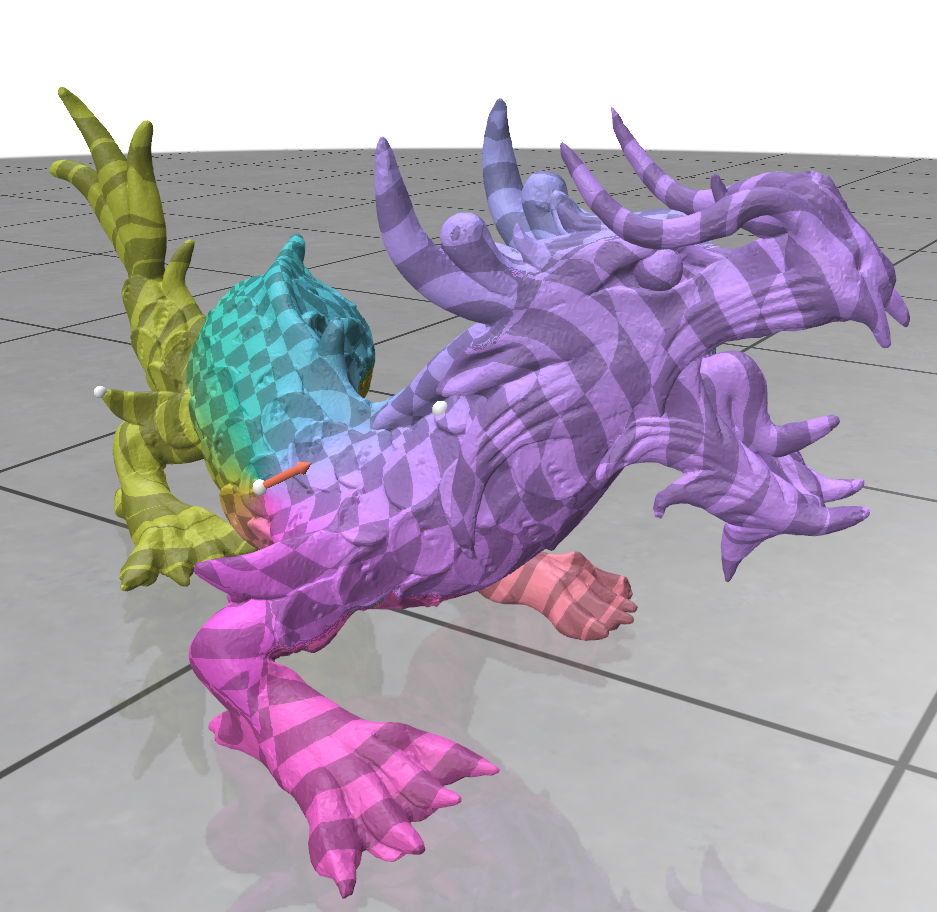
\includegraphics[width=0.5\textwidth]{dragon_log_map.png}
  \caption{\textbf{Logarithmic map on a curved surface}. \textmd{The logarithmic map provides a coordinate system on the surface with respect to an origin and a choice of an initial unit vector to define $\varphi$.}}
  \label{fig:logarithmic_map}
\end{figure}


\subsubsection{Karcher means and geometric medians on general surfaces }
A general notion of center can be defined on shapes as the point that minimize an energy which depends on its geodesic distances to all points of the set. 
Let $y_1$, $y_2$, ..., $y_n$ be a set of points on a surface $M$, the kercher mean is the point that minimizes the following energy:
$$E(x):=\frac{1}{2n}\sum_{i=1}^{n}d(x,y_i)^2$$

The gradient at a point $x$ of the energy to minimize is just the mean of the logarithms $\log_x y_i$ of the points of the set. To find the mean, $x$ can be iteratively updated to $\exp_{x}(\tau v)$ with $v=\frac{1}{n}\sum_{i=1}^{n}\log_x(y_i)$. However, it requires to compute the logarithmic map at each iteration. Thus, a fast and accurate parallel transport method would allow the computation of the mean using the logarithmic maps.


\section{Methodologies}
Let $M$ be a Riemannian manifold with metric $g$. We denote by $d(x,y)$ the corresponding geodesic distance between any pair of point $x,y$. 
The cut locus of a point $p$ on $M$ is the closure of the set of all other points on $M$ that are connected to $p$
by two or more distinct shortest geodesics. More generally, the cut locus of a closed set $X$ on $M$ is the closure of the set of 
all other points on the manifold connected to $X$ by two or more distinct shortest geodesics.

\subsection{Scalar heat method}
The Scalar Heat Method (\cite{Crane:2017:HMD}) is presented in algorithm \ref{algo2}: the heat equation and the Poisson equation are used to find the geodesic distances
between any point on the domain and the input source set. In the following, 

\begin{algorithm}
  \caption{Scalar Heat Method} \label{algo2}
  \begin{algorithmic}
    \Require A given source set in a setting where a gradient operator $\nabla$, a divergence operator $\nabla$ and a Laplace operator $\Delta = \nabla \cdot \nabla$ 
    are well defined. 
    \Ensure The distance function $d$ between any point and the source set. \\
    \noindent \textbf{I.} Integrate the heat flow $\dot{u} = \Delta u.$\\
    \textbf{II. }Evaluate the vector field $X = -\frac{\nabla u_t}{|\nabla u_t|}.$ \\
    \textbf{III. }Solve the Poisson equation $\Delta \phi = \nabla \cdot X. $\\
    \textbf{IV. } Shift $\phi$ such that the smallest distance is zero. \\
  \end{algorithmic}
\end{algorithm}
The initial conditions, the time discretization and spatial discretization can be taken as the same as in the Vector Heat Method presented below. 
\subsection{Vector heat method}
The Vector Heat Method (\cite{Sharp:2019:VHM}) is presented in algorithm \ref{algo1}: the vector heat equation is used to diffuse the input vector field and then the scalar heat vector is used to adjust the magnitude of the resulting vectors. Indeed, the vector heat equation gives vectors pointing to the right directions for small values of time $t$ but the magnitudes are wrong. 

\begin{algorithm}
\caption{Vector Heat Method} \label{algo1}
\begin{algorithmic}
\Require A vector field $X$ supported on a subset $\Omega \subset M$ of the domain $M$.
\Ensure A vector field $\overline{X}$ on all of $M$.
%\Input{A vector field $X$ supported on a subset $\Omega \subset M$ of the domain $M$.}
%\Output{A vector field $\overline{X}$ on all of $M$.}

\noindent \textbf{I.} Integrate the vector heat flow $\frac{d}{dt} Y_t = \Delta Y_t$ for time $t$, with $Y_0 = X$. \\

\textbf{II.} Integrate the scalar heat flow $\frac{d}{dt} u_t = \Delta u_t$ for time $t$, with $u_0 = |X|$. \\

\textbf{III.} Integrate the scalar heat flow $\frac{d}{dt} \phi_t = \Delta \phi_t$ for time $t$, with $\phi_0 = \mathbf{1}_{\Omega}$. \\

\textbf{IV.} Evaluate the vector field $\overline{X}_t = \frac{u_t Y_t}{\phi_t |Y_t|}$.
\end{algorithmic}
\end{algorithm}

\subsubsection{Step 1: get the right directions}
As mentioned earlier, the idea of the vector heat method is to use the vector heat equation 
\begin{equation} \label{eq:vector-heat}
  \frac{d}{dt} X_t = \Delta^\nabla X_t
  \end{equation}
to diffuse the initial vector field. The symbol $\Delta^\nabla$ denotes the connection Laplacian associated to the Levi-Civita connection $\nabla$. 
We now consider a fundamental solution to the heat equation: the \textbf{heat kernel} denoted by $k_t^\nabla$. $k_t^\nabla(x,y)$ describes how 
a vector at a single point $x$ will diffuse to all other points $y$ over time $t$. For $y$ not on the cut locus of $x$, the following asymptotic
expansion holds:
\begin{equation} \label{eq:asymptotic_expansion}
  k_t^\nabla(x, y) \sim \frac{e^{-\frac{d(x, y)^2}{4t}}}{(4 \pi t)^{n/2} j(x, y)^\frac{1}{2}} 
\left( \sum_{i=0}^{\infty} t^i \Psi_i(x, y) \right)
  \end{equation}
where the functions $\Psi_i$ are maps taking vector at $x$ to vectors at $y$. Most importantly, we have that the first function in this series 
is equal to:
$$\Psi_0(x,y) = P_{\gamma_{x\rightarrow y}}, $$ where $\gamma_{x \rightarrow y}$ is the shortest geodesic from $x$ to $y$ and $P_\gamma(X)$
denotes the parallel transport of X along $\gamma$. Thus, by taking $t\rightarrow 0$, the terms for which $i\neq 0$ vanish, so \textbf{the vector heat 
kernel is asymptotically equal up to a constant to the parallel transport along shortest paths.} This explains the step 1 of the algorithm, whose goal 
is to get the right directions of the parallel transport of the input vector field. In the following, we denote by $Y$ the solution of the 
vector diffusion equation 
\begin{align*}
  \begin{cases}
  \frac{d}{dt}Y_t  = \Delta^\nabla Y_t \\
  Y_0  = X.
\end{cases}
\end{align*}


\subsubsection{Step 2: get the right magnitudes}
We use scalar interpolation to scale the vectors obtained in step 1 and get the right magnitudes. Assume we have a collection of sources
$p_1, \dots, p_n \in M$ and associated values $u_1, \dots, u_n \in \mathbb{R}$. We define the functions $u$ and $\Phi$ 
as the solutions of two independent heat equations with initial conditions:
\begin{align}
  u(t = 0, p) = \sum_{i = 1}^nu_i\delta_{p_i}(p) \label{eq:initial_condition_1}\\
  \Phi(t = 0, p) = \sum_{i=1}^n\delta_{p_i}(p) \label{eq:initial_condition_2}
\end{align}
We then take as interpolant of the right magnitudes 
\begin{equation}
  \overline{u}(t,p) = \frac{u(t,p)}{\Phi(t,p)}
\end{equation}
In the following, we generalize the source set to any subset $\Omega \subset M$
and so the initial conditions \ref{eq:initial_condition_1} and \ref{eq:initial_condition_2}
are slightly modified to 
\begin{align*}
  u(t=0, p) = | X(p) | \\
  \Phi(t=0, p) = \mathbf{1}_{\Omega}(p)
\end{align*}

\subsubsection{Step 3: getting the final transported vector field}
The final step is simply to normalise the vector obtained in step 1 and scale them by the magnitudes obtained in step 2: 
$$\overline{X}_t(p) = \frac{\overline{u}(t,p)Y_t(p)}{|Y_t(p)|}$$ with $\overline{u}(t,p) = \frac{u(t,p)}{\Phi(t, p)}$.

\subsection{Discretization}
The vector heat method is is discretized on triangle meshes denoted by $K = (V, E, F)$
with $V$ being the set of vertices, $E$ being the set of edges and $F$ 
being the set of corresponding faces. The discretization formalism relies 
on results presented in articles \cite{10.1145/2461912.2462005} and \cite{Knoppel:2015:SPS}. Let $k,l$ be the vertices opposite 
a given edge $ij$. Denote by $ikj$ the triangle with vertices $i, j, k \in V$ and $\theta_k^{ij}$ the angle at 
vertex $k$ whose opposite edge is $ij\in E$. Likewise, we define $\theta_i^{jk}$ 
and $\theta_j^{ik}$ as the angles at vertices $i$ and $j$ whose opposite edges are $jk, ik \in E$. 
Let $a = \cot \theta_i^{jk}$, $b = \cot \theta_j^{ki}$ and $c = \cot \theta_k^{ij}$. 
\subsubsection{Discrete Laplace-Beltrami operator $\Delta$}
The Laplace Beltrami operator $\Delta$ is discretized into a weighted graph Laplacian $L\in \mathbb{R}^{|V|\times |V|}$.
$L$ is constructed such that if the triangle $ijk$ is in entry, then 
$$L_{ijk} = -\frac{1}{2}\begin{pmatrix}
  b + c & -c & -b \\
  -c & c + a & -a \\
  -b & -a & a + b
  \end{pmatrix}.$$

\subsubsection{Discrete connection Laplacian $\Delta^\nabla$} The discretized connection Laplacian 
$\Delta^\nabla$ is given by $L^\nabla \in \mathbb{C}^{|V|\times|V|}$. We define 
$\phi_{ij}$ as the rotation angle that separates a canonical edge $ij_0$ to the edge
$ij$ in the counter-clockwise order. Let $r_{ij} = e^{i((\phi_{ji} + \pi) -  \phi_{ij})}$.
Then, $$
L^\nabla_{ijk} = -\frac{1}{2}\begin{pmatrix}
  b + c & -cr_{ij} & -br_{ik} \\
  -cr_{ji} & c + a & -ar_{jk} \\
  -br_{ki} & -ar_{kj} & a + b
  \end{pmatrix}.
$$
\subsubsection{Intrinsic Delaunay triangulation} To improve robustness and accuracy, the vector heat method is first applied to a 
slightly modified mesh and the solution is then copied back to the original mesh. The intrinsic Delaunay mesh prevents from getting 
negative diagonal terms in the local $3\times3$ matrices $L_{ijk}$ and $L^\nabla_{ijk}$. To do that, the intrinsic Delaunay algorithm 
"flips" any edge $ij$ where $\theta_k^{ij} + \theta_l^{ji}>\pi$: the edge $ij$ is replaced by the new edge $kl$, with $k,l$ being the 
vertices opposite the edge $ij$. Additionally, the angles encoding the direction of the flipped edge $kl$ at vertices $k,l$ are computed 
so that the local tangent spaces can be updated on each flip and so that the solution computed on Delaunay triangulation can be easily mapped 
back to the original mesh thanks to local polar coordinates. 

\subsubsection{Discretized equations}
Let $A_{ijk}$ be the area of the triangle $ijk$. We define the \textbf{lumped mass matrix} $M$ which is the diagonal matrix of shape $|V| \times |V|$ with diagonal terms 
equal to $$M_{i,i} = \frac{1}{3}\sum_{ijk\in F}A_{ijk}.$$ Applying a one-step backward Euler approximation gives the following equations of for the first three points 
of algorithm \ref{algo1}:
\begin{align*}
 (M-tL^\nabla)Y & = Y_0 \\
 (M - tL)u & = u_0 \\
 (M - tL)\phi & = \phi_0
\end{align*}
with the source data represented in $Y_0\in \mathbb{C}^{|V|}$, $u_0 \in \mathbb{R}^|V|, \phi_0 \in \mathbb{R}^{|V|}$.
\begin{comment}
\begin{algorithm}
\caption{An algorithm with caption}\label{alg:cap}
\begin{algorithmic}
\Require $n \geq 0$
\Ensure $y = x^n$
\State $y \gets 1$
\State $X \gets x$
\State $N \gets n$
\While{$N \neq 0$}
\If{$N$ is even}
    \State $X \gets X \times X$
    \State $N \gets \frac{N}{2}$  \Comment{This is a comment}
\ElsIf{$N$ is odd}
    \State $y \gets y \times X$
    \State $N \gets N - 1$
\EndIf
\EndWhile
\end{algorithmic}
\end{algorithm}
\end{comment}

\section{Experiences}

\subsection{Our set-up}
To realize these experiences, we first tested the C++ demo presented in the paper's website.
In this demo, the solvers for the scalar and vector heat methods were implemented in a library named Geometry Central.
To simplify the experimentation and work in a more familiar set-up, we used instead a Python library equivalent named Potpourri3d \cite{library_potpourri3d}, 
which was developped by Nicolas Sharp, one of the authors of the paper.
In addition to this, we used Trimesh for the manipulation of meshes and PyVision to visualize the results.
For the 3d bodies used throught the experiment, we mainly used those in the github repository~\cite{github_objects_repo},
as they presented clean 3d manifolds.

A fraction of the meshes used contained some degenerations present in the form of duplicate edges, disconections or isolated vertices.
This required an extra step in the preprocessing before applying the algorithms. The first step consisted in the union of all vertices in
an epsilon distance from one another, which removed disconections. Then we removed unreferenced vertices to avoid isolated ones. And finally,
for the duplicated edges, we did a more manual approach by analyzing the origin of the errors and removed the faces that generated the issue. 

\subsection{Scalar heat robustness}

The first experience we did was to analyze the robustness of the Scalar Heat Method (shm)~\cite{Crane:2017:HMD}. In
the original paper, the authors tested different noise types: missing and sliver triangles,
noisy coordinates and smoothed surfaces. So we recreated similar perturbations and numerically
measured the results.

For this numerical representation, we decided to compare two things. First, the original body
with an exact slower method from the gdist library~\cite{exact_method_algorithm}\cite{exact_method_library}
against the noisy body with the scalar heat method.
Then, the noisy body with the exact method against the noisy body with the scalar heat method again.
The first values explain the imperfections comming from the inexact method and the noise, while
the second only tests the behaviour of our method in a noisy environment.

Given $M = (V, F)$ our original mesh, $N = |V|$ the number of vertices in the mesh, and $\hat{M} = (\hat{V}, \hat{F})$ the noisy mesh,
the formulas used for this representation were:

\begin{equation} \label{eq:nvn_precision}
  \text{precision}_{\text{noisy v noisy}} = \frac{\sum_{i=1}^N \mathbf{1}_{\{|\text{dist}_1(\hat{V}_i) - \text{dist}_2(\hat{V}_i)| < 2\%\}}}{\text{N}} 
\end{equation}

\begin{equation} \label{eq:ovn_precision}
  \text{precision}_{\text{original v noisy}} = \frac{\sum_{i=1}^N \mathbf{1}_{\{|\text{dist}_1(V_i) - \text{dist}_2(\hat{V}_i)| < 2\%\}}}{\text{N}} 
\end{equation}

Where $\text{dist}_1$ and $\text{dist}_2$ are both the normalized distances (from 0 to 1 for the intrinsic farthest point) obtained from the exact method and the shm respectively.

We tested the robustness with two different type of noises (Fig~\ref{fig:all_bunnies}), inspired from what was presented in the paper. 
The first one is a gaussian perturbation of the position of all vertices. The variation of this noise was the noise level times the average edge length.
The second noise was a triangle swapp and triangle removal of a percentage of all triangles.
The triangle swap is simply to find a pair of faces $abc$, $bcd$ and convert them to $abd$ and $acd$.
This last perturbation quickly degenerated the meshes to the point where the exact algorithm could not
process the geodesic distances, so it was keept to a smaller noise level. 

To have a more general analysis, we used three different meshes and a set of ten random
source points. The meshes from the repo~\cite{github_objects_repo} were, in order of complexity, cow (5.8k triangles), the Stanford Bunny (69.5k triangles) and Horse (97k triangles).

In fig~\ref{fig:original_vs_noisy} we have the precision of the shm on noisy mesh compared with the exact method in the original mesh for
different levels of gaussian noise, while in fig~\ref{fig:noisy_vs_noisy} we compare both methods only in the noisy objects.

We can see for the the large meshes the precision starts being virtually perfect, but it
decays gradually with the noise increases. This appears only on the first graph, as if we compare it to the noisy vs noisy, the precision
only decays slightly for the noisiest tests. We can understand that most of these errors come from comparing the original and the noisy objects
and do not depend on the method used.

For smaller meshes, where the edge-length body-length ratio is more significant, we have that the precision is generally smaller,
and even comparing both methods on the same noisy object gives a more significant number of inaccuracies, ranging from 10\% for the
original object to 30\% for the largest noise levels.

Analyzing the errors for the swapped and missing faces noise we plot our results
in fig~\ref{fig:noisy_vs_noisy_swapped_and_removed}. We see that SHM is virtually perfect
for larger meshes, but again the noise on the smaller model is more significant because
of its simplicity, what leads to some imprecisions. 

\begin{figure}
  \centering
  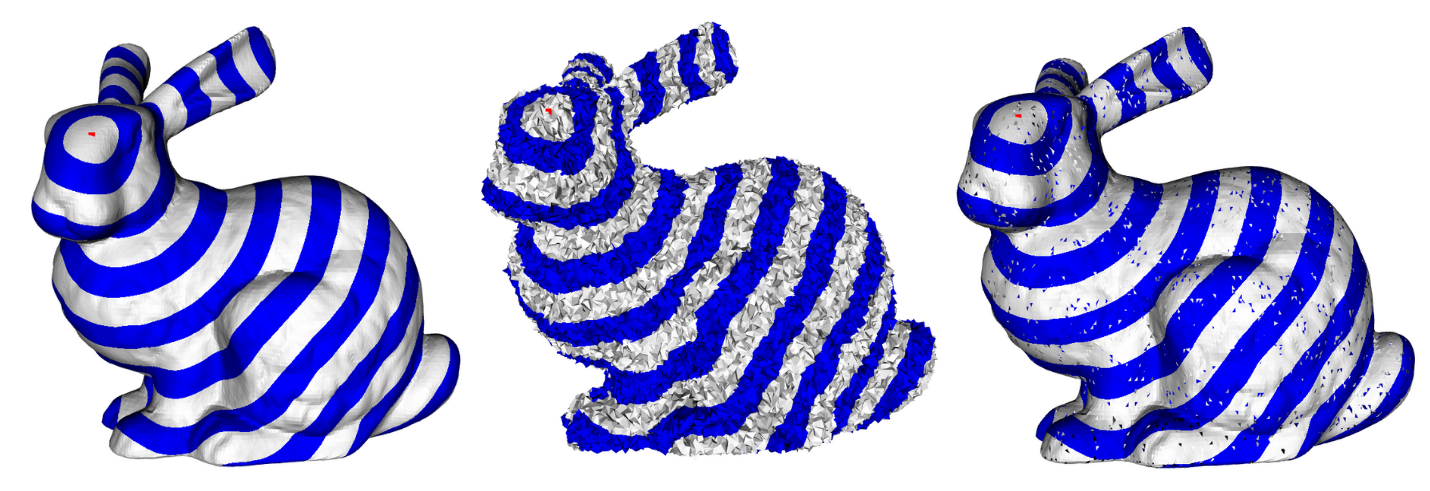
\includegraphics[width=8cm]{all_bunnies.png}
  \caption{From left to right we have the original stanford-bunny, the gaussian noised (50\% of average edge length) and a triangle swapped and removed noise (5\% of all triangles affected)}
  \label{fig:all_bunnies}
  \Description{}
\end{figure}

\begin{figure}[htbp]
  \centering
  \hfill
  \begin{subfigure}[b]{0.23\textwidth}
    \centering
    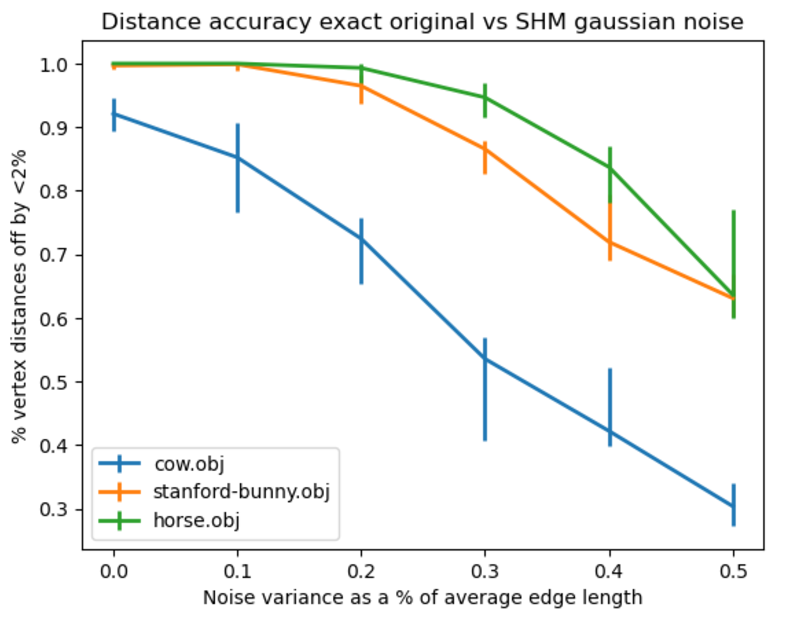
\includegraphics[width=\textwidth]{original_vs_noisy.png}
    \caption{Original vs noisy meshes}
    \label{fig:original_vs_noisy}
  \end{subfigure}
  \begin{subfigure}[b]{0.23\textwidth}
    \centering
    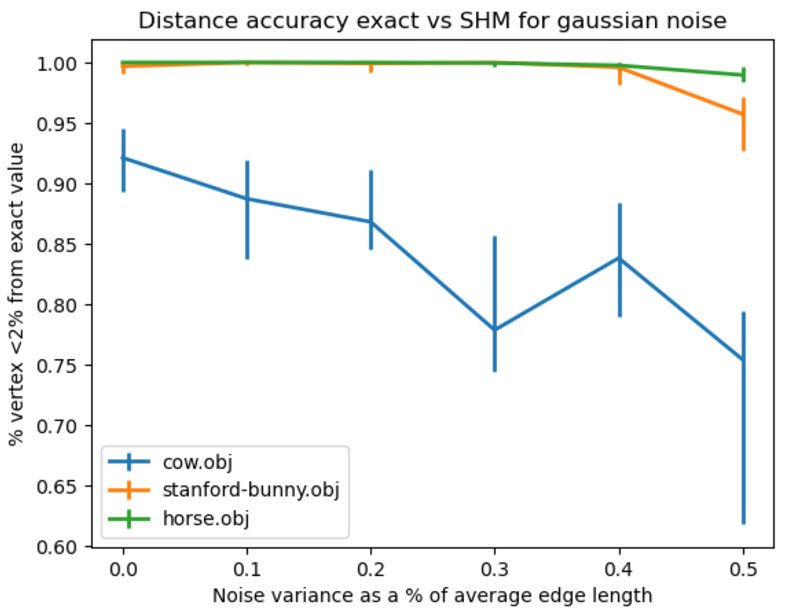
\includegraphics[width=\textwidth]{noisy_vs_noisy.png}
    \caption{Noisy vs noisy meshes}
    \label{fig:noisy_vs_noisy}
  \end{subfigure}
  \caption{Precision comparison with Gaussian noise}
  \label{fig:original_vs_noisy_gaussian}
  \Description{}
\end{figure}

\begin{figure}
  \centering
  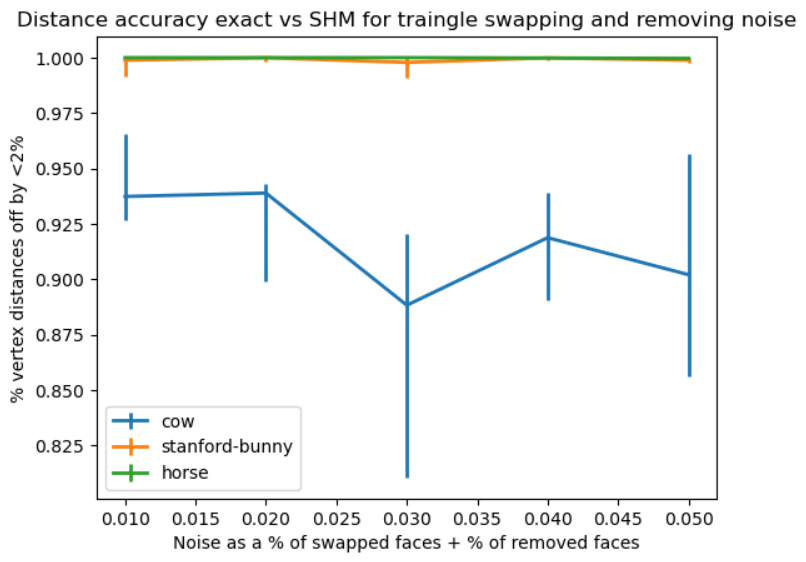
\includegraphics[width=8cm]{original_vs_original_swapped_and_removed_triangles.png}
  \caption{Noisy vs noisy meshes for swapped and removed faces noise type}
  \label{fig:noisy_vs_noisy_swapped_and_removed}
\end{figure}

Lastly, one type of noise for triangle meshes that was not introduced in the paper comes from
wrongly connected faces (Fig~\ref{fig:hands}). The algorithm presented is not inmune to these errors,
as it gives a correct representation of the distance for the perturbed mesh. So the method
presented is relatively robust to noise, but it still requires a curated mesh as its input. 

One possible solution to this is to take a point cloud instead. If the manifold represented is
dense enough, it will give a correct representation of the distances (Fig~\ref{fig:hand_distances}).

\begin{figure}
  \centering
  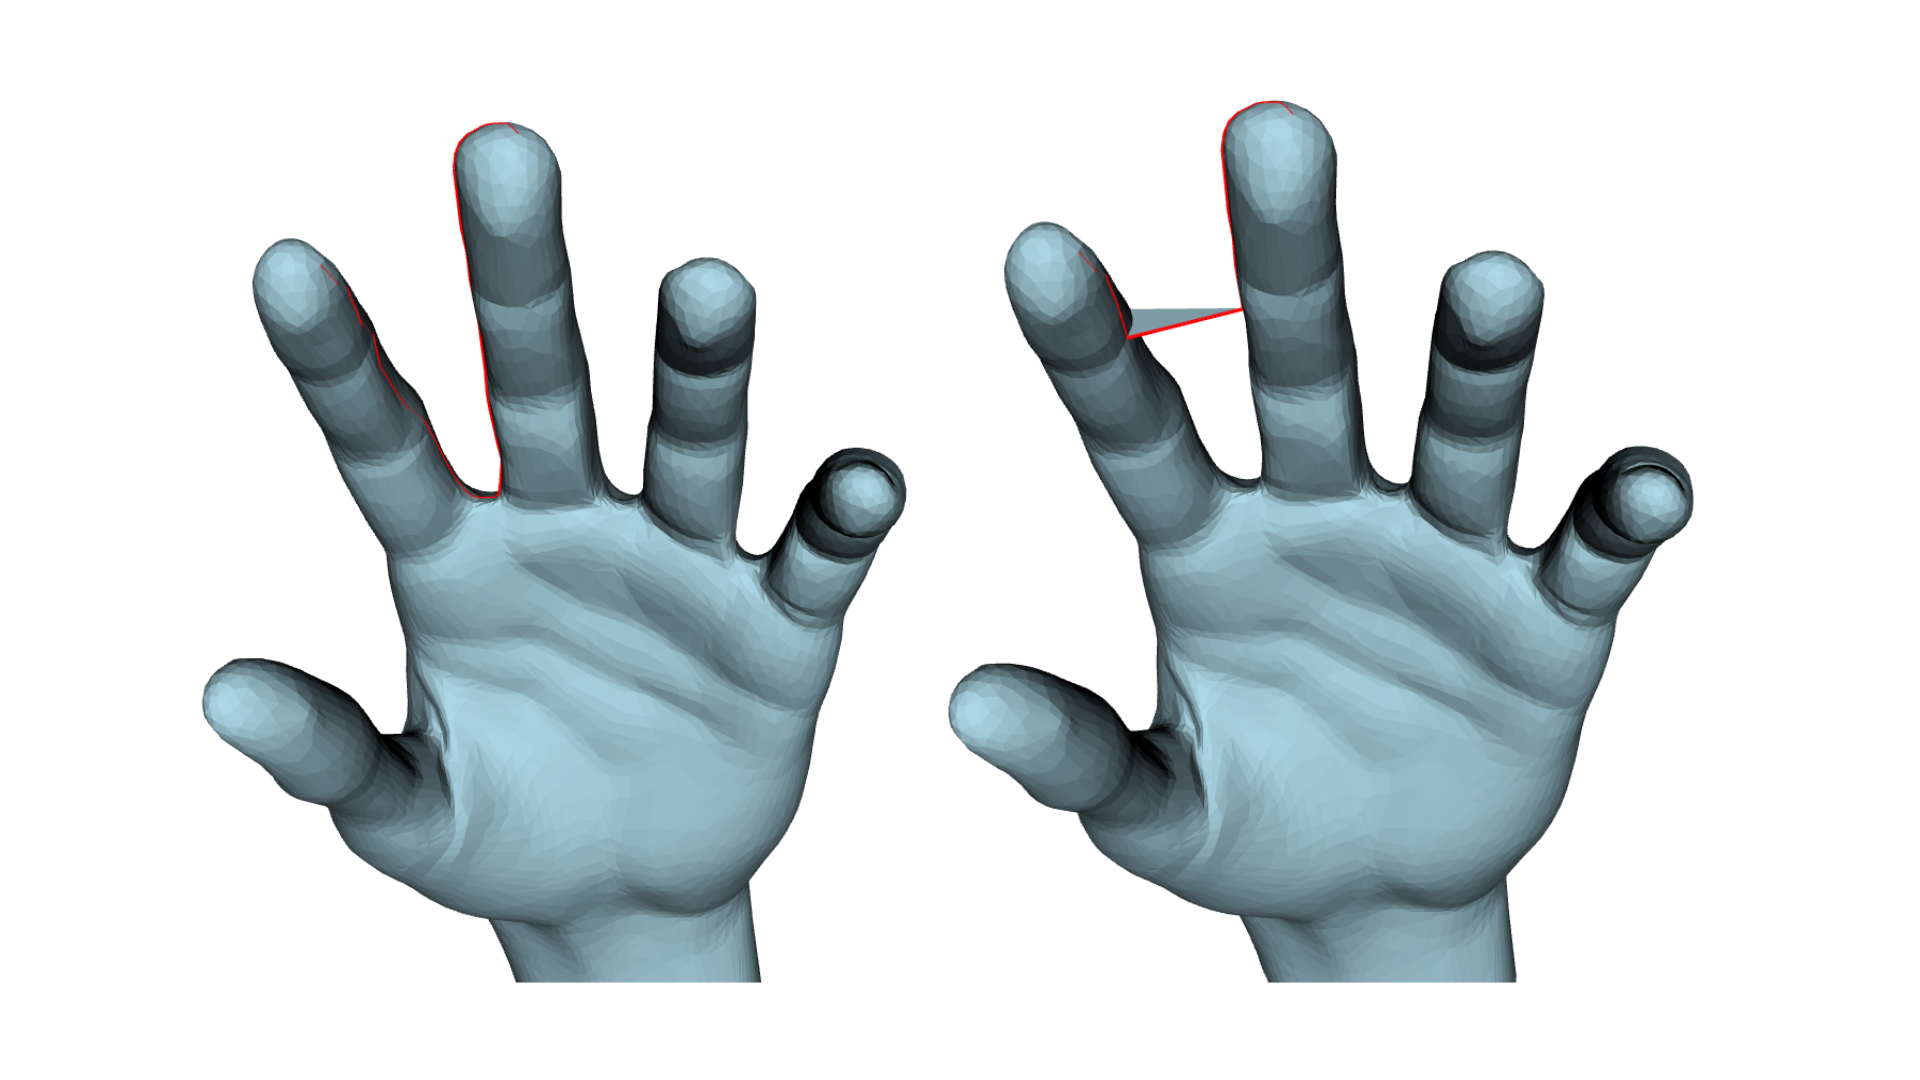
\includegraphics[width=8cm]{hands.png}
  \caption{Shortest path from fingertip to fingertip with and without an additional incorrect face}
  \label{fig:hands}
\end{figure}

\begin{figure}
  \centering
  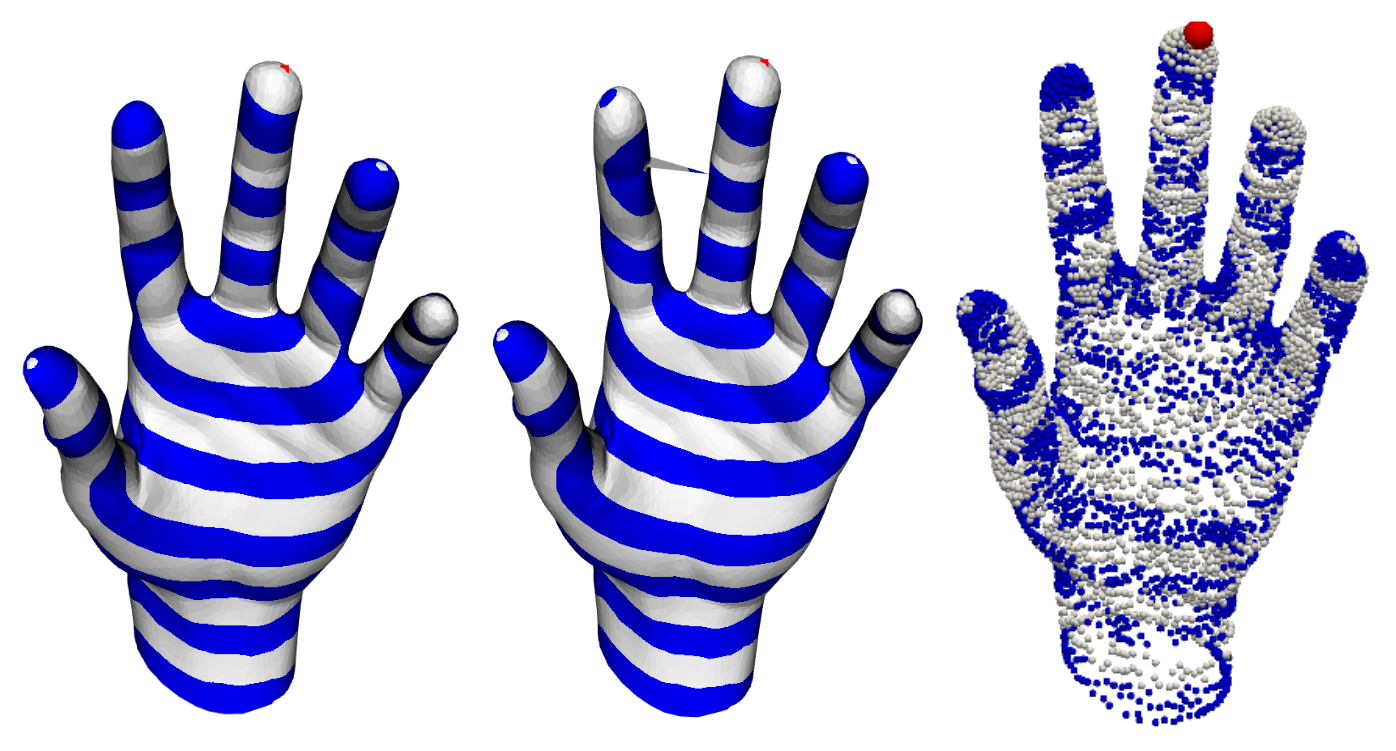
\includegraphics[width=8cm]{hands_distances.png}
  \caption{Distances from fingertip in original hand mesh, perturbed mesh and point cloud}
  \label{fig:hand_distances}
\end{figure}

\subsection{Behavior at cut locus}
(cécile)
Because there is the ambiguity of choosing which closest point in $\Omega$ to take for points on the cut locus, we decided to check 
the behaviour of the vector heat method on these points. For simplicity, $\Omega$ was restricted to a set a two source points $p_1, p_2$ and 
the experiments were conducted on the same meshes mentioned above: the cow, the stanford bunny and the horse. We first used the heat method for 
distance computation defined in \cite{crane_geodesics_2013} to compute the geodesic distances from our two points. The cut locus
points were detected by setting a threshold to $\epsilon$ and looking at the vertices $p$ such that $|d(p_1, p) - d(p_2, p)|<\epsilon$. We then 
observed the behaviour of the vector heat method at these points for $p_1, p_2$ sampled at random. Every time, the method yielded the result that 
we expected. This can be explained by the fact due to the discretisation and the computation precision of the geodesic distances, the cut locus 
points that are detected are not really on the cut locus, but only close to cut locus points. In theory, for points which are really on the cut 
locus, the diffused vectors should be an average of all the closest vectors. In figures \ref{fig:cut_locus_vectors}, you can see that
the "cut locus" vectors constitute a non-continuity of the vector field but they all point to the right directions. 


%\begin{comment}
\begin{figure}[htbp]
  \centering
  \hfill
  \begin{subfigure}[b]{0.23\textwidth}
    \centering
    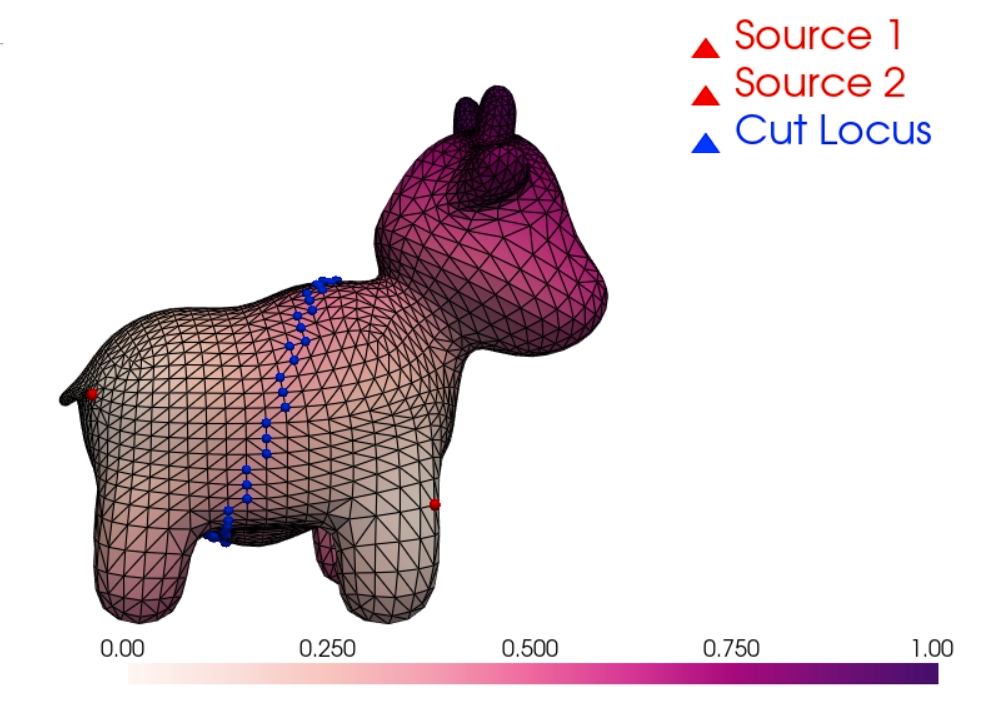
\includegraphics[width=\textwidth]{img/cut_only_distances_pink.png}
    \caption{Geodesic distances on the cow mesh}
    \label{fig:cut_locus_only_distances}
  \end{subfigure}
  \begin{subfigure}[b]{0.23\textwidth}
    \centering
    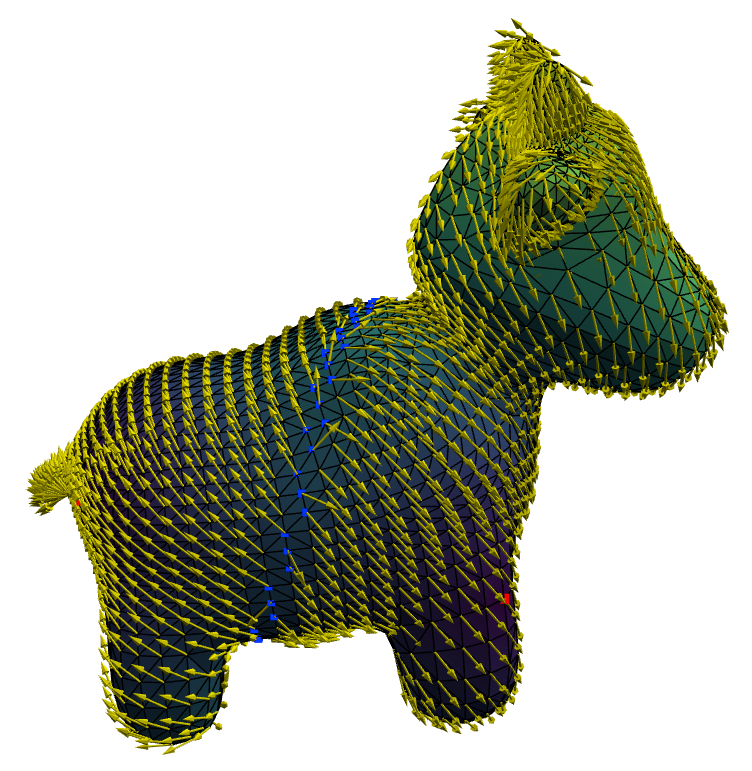
\includegraphics[width=0.7\textwidth]{img/cow_cut_locus_vectors.png}
    \caption{Cut locus vectors on the cow mesh}
    \label{fig:cut_locus_cow_vectors}
  \end{subfigure}
  \caption{Vector heat method on pseudo cut locus points}
  \label{fig:cut_locus_vectors}
\end{figure}

\subsection{Log-map recreation}

We attempted to implement the steps necessary to add a specific image
on the surface of a manifold. This is done through the Log-map function.
This function takes as input a mesh and an initial vertex and outputs
the reference of each point on a 2d plane. This in practice can be used to
plot any image on the surface.

We recreated the setup to try to plot a logo on the chest of a 3d model
(fig~\ref{fig:low_poly_human}). In this attempt we transported, scaled and rotated a
2d image from a jpg onto the front of the model and we painted each
vertex of its respective color. The color in each face was a gradient from
the vertice colors, so the result was a blurried low-resolution image. 

To solve this issue, we re-attempt with a higher-poly model (450k triangles) (fig~\ref{fig:high_poly_human}),
but this time the log-solver could not reliably obtain the correct values due to the complexity of the model
and high triangle count. This can be verified by using the original log-map
picture and their demo (fig~\ref{fig:high_poly_human_original_demo}).

We finally attempted with no succes no use pyvista to add a texture on each face
to obtain a higher resolution picture from a low-poly mesh. This would maintain
the good behavior of the algorithm on the lower-poly body, while allowing to
have details in the image too. 

\begin{figure}
  \centering
  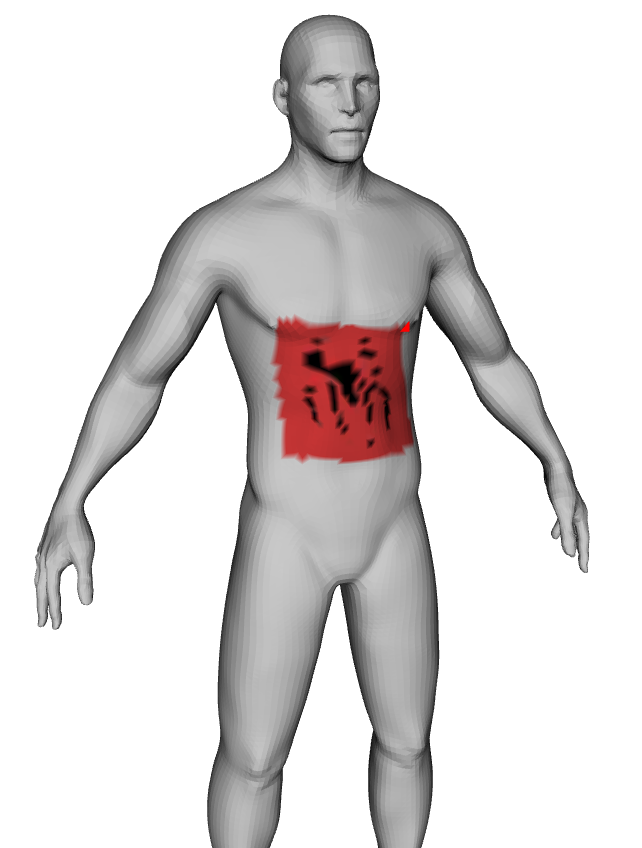
\includegraphics[width=4cm]{human_spiderman.png}
  \caption{Low-poly human (50k triangles) log-map test}
  \label{fig:low_poly_human}
\end{figure}

\begin{figure}[htbp]
  \centering
  \hfill
  \begin{subfigure}[b]{0.23\textwidth}
    \centering
    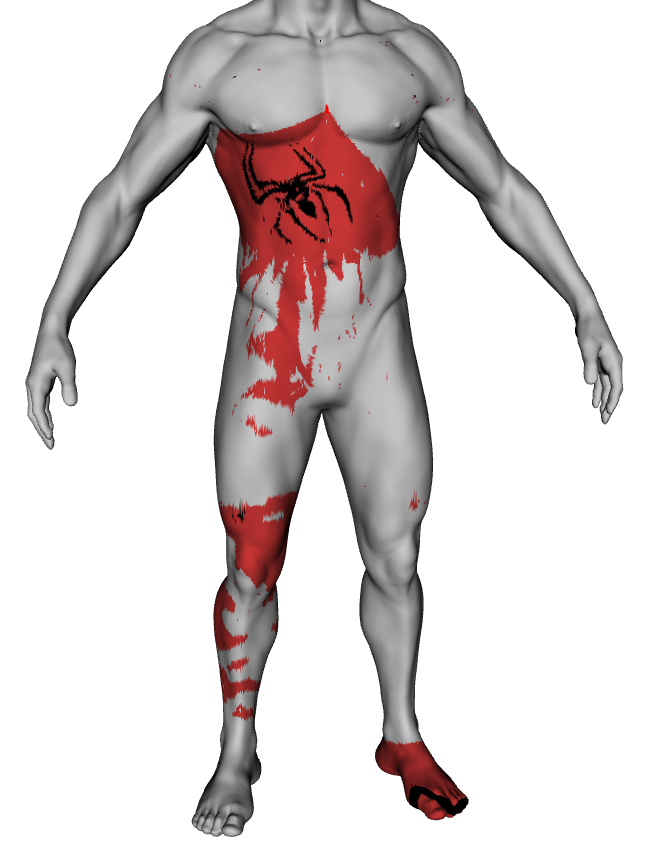
\includegraphics[width=4cm]{human_spiderman_high.png}
    \caption{High-poly human log-map test}
    \label{fig:high_poly_human}
  \end{subfigure}
  \begin{subfigure}[b]{0.23\textwidth}
    \centering
    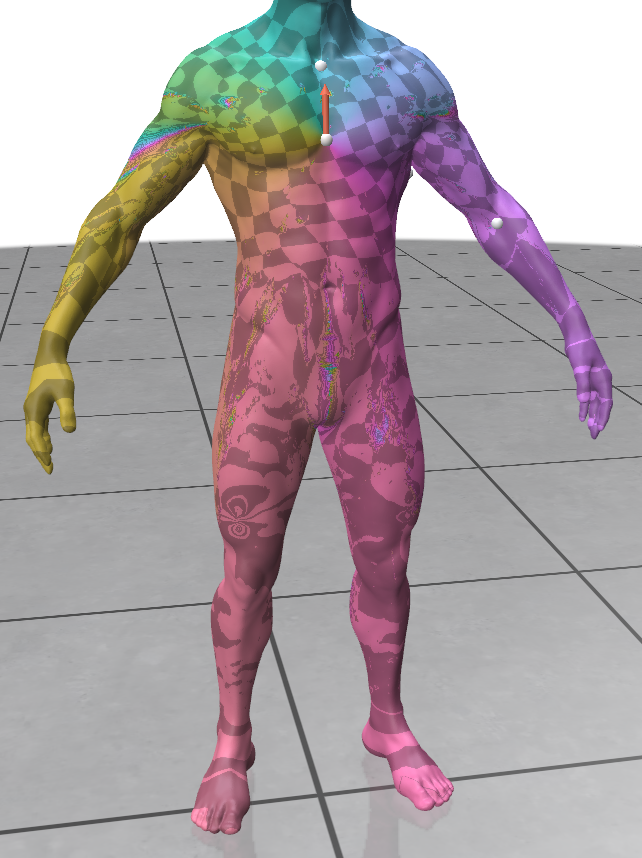
\includegraphics[width=4cm]{log_map_wrong.png}
    \caption{High-poly human log-map with original demo}
    \label{fig:high_poly_human_original_demo}
  \end{subfigure}
  \caption{Log-map on high-poly mesh (450k triangles)}
  \label{fig:cut_locus_vectors}
\end{figure}

\subsection{Preprocessing vs processing times}

The implementation of the SHM algorithm is composed of two parts:
a preprocessing to get the laplacians, and the computation of the 
distances from a source vertex/set of vectors. In this point we wanted to compare the speed of this method with
the exact method using meshes of different sizes. 

For the experiment, we ran three tests. First, we measured the time for the exact method,
then we measured the time for the SHM executing the preprocessing and processing
every loop, and finally we executed the SHM preprocessing once and then we only computed
the distances in the loop. We plotted the results obtained in fig~\ref{fig:time_graphs}. 

We can see that for the larger plots the exact algorithm is slower than the SHM. 
However, almost all of the time is dedicated to the preprocessing of the mesh, 
so the real advantage of the method is for the case where we work with a limited
quantity of meshes that we have preprocess beforehand. Moreover, we did not
use the Fast marching method for the comparaisson due to complications on its
implementation in python, so there is probably an even smaller time gain for using
the SHM if we compare it with non-exact fast methods.

\begin{figure}
  \centering
  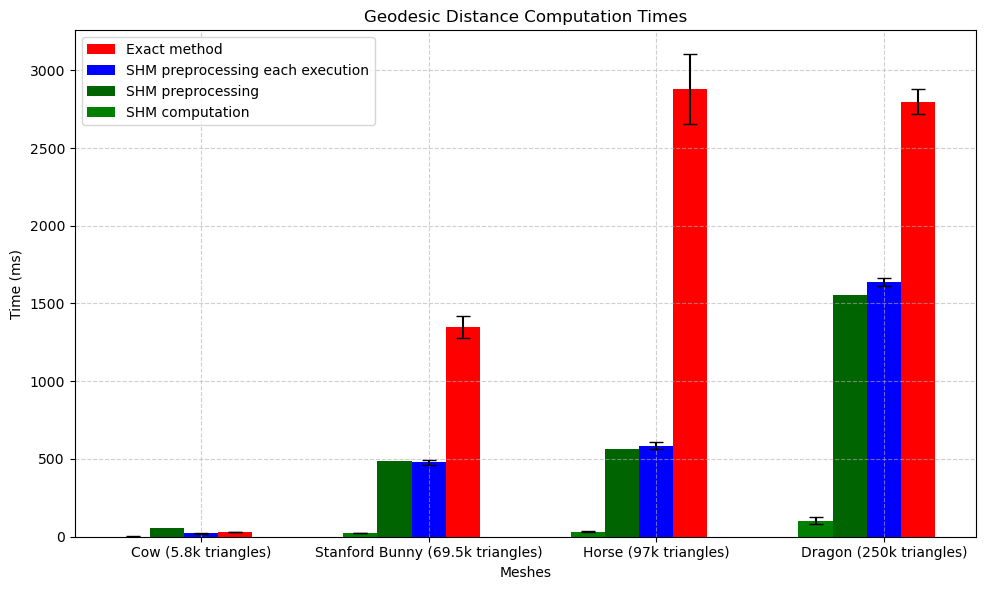
\includegraphics[width=8cm]{time_graphs.png}
  \caption{Times measured}
  \label{fig:time_graphs}
\end{figure}

\section{Conclusion}

In this paper, we have presented the Vector Heat Method, a fast and accurate method to parallel transport a vector field on a curved surface.

\bibliographystyle{ACM-Reference-Format}
\bibliography{ref}


\end{document}

\endinput
